% Options for packages loaded elsewhere
\PassOptionsToPackage{unicode}{hyperref}
\PassOptionsToPackage{hyphens}{url}
\documentclass[
]{article}
\usepackage{xcolor}
\usepackage{amsmath,amssymb}
\setcounter{secnumdepth}{-\maxdimen} % remove section numbering
\usepackage{iftex}
\ifPDFTeX
  \usepackage[T1]{fontenc}
  \usepackage[utf8]{inputenc}
  \usepackage{textcomp} % provide euro and other symbols
\else % if luatex or xetex
  \usepackage{unicode-math} % this also loads fontspec
  \defaultfontfeatures{Scale=MatchLowercase}
  \defaultfontfeatures[\rmfamily]{Ligatures=TeX,Scale=1}
\fi
\usepackage{lmodern}
\ifPDFTeX\else
  % xetex/luatex font selection
\fi
% Use upquote if available, for straight quotes in verbatim environments
\IfFileExists{upquote.sty}{\usepackage{upquote}}{}
\IfFileExists{microtype.sty}{% use microtype if available
  \usepackage[]{microtype}
  \UseMicrotypeSet[protrusion]{basicmath} % disable protrusion for tt fonts
}{}
\makeatletter
\@ifundefined{KOMAClassName}{% if non-KOMA class
  \IfFileExists{parskip.sty}{%
    \usepackage{parskip}
  }{% else
    \setlength{\parindent}{0pt}
    \setlength{\parskip}{6pt plus 2pt minus 1pt}}
}{% if KOMA class
  \KOMAoptions{parskip=half}}
\makeatother
\usepackage{graphicx}
\makeatletter
\newsavebox\pandoc@box
\newcommand*\pandocbounded[1]{% scales image to fit in text height/width
  \sbox\pandoc@box{#1}%
  \Gscale@div\@tempa{\textheight}{\dimexpr\ht\pandoc@box+\dp\pandoc@box\relax}%
  \Gscale@div\@tempb{\linewidth}{\wd\pandoc@box}%
  \ifdim\@tempb\p@<\@tempa\p@\let\@tempa\@tempb\fi% select the smaller of both
  \ifdim\@tempa\p@<\p@\scalebox{\@tempa}{\usebox\pandoc@box}%
  \else\usebox{\pandoc@box}%
  \fi%
}
% Set default figure placement to htbp
\def\fps@figure{htbp}
\makeatother
\setlength{\emergencystretch}{3em} % prevent overfull lines
\providecommand{\tightlist}{%
  \setlength{\itemsep}{0pt}\setlength{\parskip}{0pt}}
\usepackage{bookmark}
\IfFileExists{xurl.sty}{\usepackage{xurl}}{} % add URL line breaks if available
\urlstyle{same}
\hypersetup{
  hidelinks,
  pdfcreator={LaTeX via pandoc}}

\author{}
\date{}

\begin{document}

\section{Finiteness for finite groups in every
characteristic}\label{finiteness-for-finite-groups-in-every-characteristic}

\emph{Written and self-checked by GPT-6.1 Sol (OpenAI) in Codex at
Ultra. Original exposition, proofs, exercises and diagrams are CC0.}

Averaging needs division by the group order. A monic polynomial whose
roots form a finite orbit needs no division at all. This change of
viewpoint proves finite generation in every characteristic, even for an
algebra with nilpotents over a Noetherian base ring. It also explains
why finding a few invariants can be enough to determine the whole ring.

All rings are commutative with identity. An algebra is \textbf{of finite
type} when finitely many elements generate it as an algebra; a module is
\textbf{finite} when it is finitely generated. An element is
\textbf{integral} over a subring if it satisfies a monic polynomial over
that subring. The field in this lesson can have any characteristic.

We use \href{NOE-INV-03.html}{Invariants of finite groups and Noether's
degree bound} and \href{NOE-INV-02.html}{Polarization, vector invariants
and symbolic evaluation}, both earlier lessons in this course. The
commutative algebra prerequisites are existing lessons in
\emph{Commutative algebra for geometry}:
\href{../AG-CA/AG-CA-03.html\#2-polynomial-rings-and-finite-geometric-descriptions}{Noetherian
and Artinian rings}, Theorem 2.1 and the
\href{../AG-CA/AG-CA-03.html\#1-three-ways-to-recognize-a-noetherian-module}{finite-submodule
criterion, Proposition 1.2}; and
\href{../AG-CA/AG-CA-05.html\#1-a-monic-equation-is-finite-control}{Integral
extensions}, Theorem 1.2, for transitivity and ``integral plus finite
type implies finite''. Their proofs are written in the programme.
Noether normalization is Corollary 3.2 of
\href{../AG-CA/AG-CA-09.html\#3-normalization-that-respects-ideals}{Krull
dimension and Noether normalization}: every finite-type field algebra is
finite over a polynomial subalgebra. We prove the additional
finite-normalization assertion here, including imperfect fields and
inseparable extensions.

\subsection{1. A monic equation from each
orbit}\label{a-monic-equation-from-each-orbit}

Let a finite group \(G\) act on a ring \(A\) by automorphisms, and write
\(B=A^G\). Repeated values in an orbit do not cause a problem: we take
one factor for each group element.

\protect\phantomsection\label{proposition-1-1}{}

\textbf{Proposition 1.1 (orbit integrality).} Every \(a\in A\) is
integral over \(B\).

\textbf{Proof.} Form \[
P_a(T)=\prod_{g\in G}(T-g(a)).
\] Every coefficient is fixed by \(G\), since applying an element of the
group permutes the factors. The polynomial is monic and \(P_a(a)=0\),
because one factor corresponds to the identity. Thus it is the required
integral equation. No cancellation or division was used. \(\square\)

Integrality by itself is weaker than finite generation. The useful extra
fact is that an algebra generated by finitely many integral elements is
a finite module. If \(a_i\) satisfies a monic equation of degree
\(d_i\), reduction by these equations shows that the products
\(\prod_i a_i^{e_i}\), \(0\leq e_i<d_i\), span the algebra as a module.
We will use this concrete spanning set twice.

\protect\phantomsection\label{theorem-1-2}{}

\textbf{Theorem 1.2 (finite-group finiteness over a Noetherian base).}
Let \(R\) be Noetherian, let \(A\) be a finite-type \(R\)-algebra, and
let \(G\) be a finite group of \(R\)-algebra automorphisms. Then
\(B=A^G\) is a finite-type \(R\)-algebra and \(A\) is finite over \(B\).

\textbf{Proof.} Choose algebra generators \(a_1,\ldots,a_s\) for
\(A/R\). Let \(C\subset B\) be the \(R\)-algebra generated by the
coefficients of their orbit polynomials \(P_{a_i}\). There are at most
\(s|G|\) such coefficients. Therefore \(C\) is of finite type over
\(R\), and is Noetherian by Hilbert basis.

Each \(a_i\) is integral over \(C\). The preceding power reduction makes
\(A=C [a_1,\ldots,a_s]\) a finite \(C\)-module. Now \(B\subset A\) is a
\(C\)-submodule: multiplication by an element of \(C\) preserves
invariance. Since \(C\) is Noetherian, this submodule is finite. Let
\(b_1,\ldots,b_r\) span it over \(C\). If \(c_1,\ldots,c_t\) generate
\(C\) over \(R\), then \[
B=R [c_1,\ldots,c_t,b_1,\ldots,b_r].
\] Indeed, the algebra on the right contains every \(C\)-linear
combination of the \(b_i\), and all its generators lie in \(B\).

The same finite \(C\)-spanning set for \(A\) also spans \(A\) over
\(B\), since \(C\subset B\). This proves both assertions. \(\square\)

This proof works when \(A\) has zero divisors or nilpotents and when the
action has a kernel. Over a field it includes all modular linear
actions. It supplies existence of a finite generating set, but its
submodule step gives no uniform upper bound on generator degrees as the
representation varies.

The construction can be visualized as a tower. Its finite assertions
come from two different mechanisms.

\begin{figure}
\centering
\pandocbounded{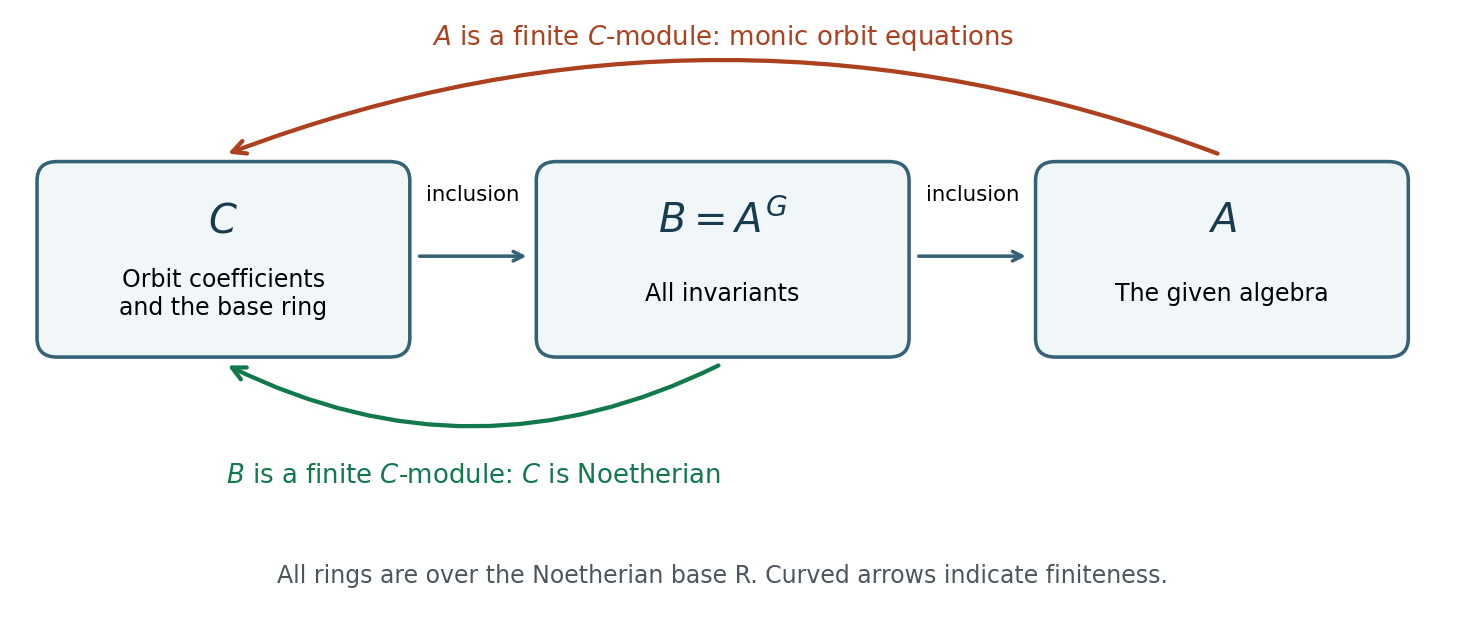
\includegraphics[keepaspectratio,alt={Tower of invariant subrings: the orbit coefficients generate C inside B=A fixed by G inside A; monic orbit equations make A finite over C, and Noetherianity makes B finite over C.}]{figures/integrality-tower.png}}
\caption{Tower of invariant subrings: the orbit coefficients generate C
inside B=A fixed by G inside A; monic orbit equations make A finite over
C, and Noetherianity makes B finite over C.}
\end{figure}

The horizontal inclusions are ring inclusions. The curved arrows
describe module finiteness over \(C\), rather than maps in the reverse
direction. All three rings are over the original base \(R\). Editable
diagram.

\subsection{2. A modular action computed without
averaging}\label{a-modular-action-computed-without-averaging}

Let \(k\) have characteristic \(p>0\), and let the cyclic group of order
\(p\) act on \(k [x,y]\) through \[
\sigma(x)=x,\qquad \sigma(y)=y+x.
\] Its effective order is \(p\). Set \[
z=y^p-x^{p-1}y.
\] The binomial identity in characteristic \(p\) shows \(\sigma(z)=z\).

\protect\phantomsection\label{theorem-2-1}{}

\textbf{Theorem 2.1.} The invariant ring is \(k [x,z]\). The ambient
polynomial ring is free of rank \(p\) over this invariant ring, with
basis \(1,y,\ldots,y^{p-1}\).

\textbf{Proof.} First \(x,z\) are algebraically independent. A nonzero
expression \(\sum_{j=0}^d c_j(x)z^j\), with \(c_d\ne0\), has
\(y\)-degree \(pd\) and leading coefficient \(c_d(x)\), so it cannot
vanish.

The monic relation \(y^p-x^{p-1}y-z=0\) reduces every polynomial to
\protect\phantomsection\label{equation-1}{}

\[
f=\sum_{j=0}^{p-1} b_j(x,z)y^j.
\tag{1}
\] This representation is unique. The leading \(y\)-degrees of
\(z^a y^j\), for \(a\geq0\) and \(0\leq j<p\), are \(pa+j\), all
distinct; choose the greatest one in any supposed nonzero relation to
obtain a contradiction. This proves the free-module assertion.

Suppose (1) is invariant. The action fixes every \(b_j\). If \(r\geq1\)
is the greatest index with \(b_r\ne0\), then \[
\sigma(f)-f=\sum_{j=1}^r b_j\bigl((y+x)^j-y^j\bigr)
\] has coefficient \(rxb_r\ne0\) at \(y^{r-1}\). Here \(1\leq r<p\), and
uniqueness of (1) applies to this expression, whose \(y\)-degree is less
than \(p\). This contradicts invariance. Thus only \(b_0\) remains,
proving the ring assertion. \(\square\)

For \(k=\mathbb F_p\), this is a modular linear action. Over
\(\mathbb F_2\), replacing \(x\) by \(y+z\) converts a swap of two
coordinates into this transvection. The exercise below carries out that
conversion.

\subsection{3. The finiteness criterion for subalgebras of a
field}\label{the-finiteness-criterion-for-subalgebras-of-a-field}

An arbitrary subalgebra of a finite-type algebra need not be of finite
type. Noether's criterion identifies an extra condition that restores
finiteness. We first supply the field argument needed to use
normalization at the full stated generality.

\protect\phantomsection\label{lemma-3-1}{}

\textbf{Lemma 3.1 (relative algebraic closure).} Let \(K/F\) be a
finitely generated field extension. The subfield \(L\) of elements of
\(K\) algebraic over \(F\) is finite over \(F\).

\textbf{Proof.} Choose a transcendence basis \(t_1,\ldots,t_r\) of
\(K/F\). Because \(K\) is finitely generated as a field, it is finite
over \(F(t_1,\ldots,t_r)\); write that degree as \(N\). For any finite
intermediate extension \(E/F\) in \(L\), the \(t_i\) remain
algebraically independent over \(E\). Otherwise a polynomial relation
with coefficients in the algebraic extension \(E\), followed by
transitivity of algebraicity, would contradict independence over \(F\).

Moreover \protect\phantomsection\label{equation-2}{}

\[
[E(t_1,\ldots,t_r):F(t_1,\ldots,t_r)]=[E:F].
\tag{2}
\] To verify (2), take an \(F\)-basis of \(E\). It spans over the
rational function field. A rational-function linear relation among its
elements clears denominators to a polynomial relation; comparison of the
coefficients of the independent monomials in the \(t_i\) proves
independence. Thus \([E:F]\leq N\), since
\(E(t_1,\ldots,t_r)\subset K\).

The degrees of finite intermediate extensions in \(L\) are consequently
bounded. Choose one, \(E_0\), with maximal degree. For every \(a\in L\),
the field \(E_0(a)\) is finite over \(F\). Maximality and the tower
formula force \(E_0(a)=E_0\). Hence \(L=E_0\) is finite. \(\square\)

\protect\phantomsection\label{lemma-3-2}{}

\textbf{Lemma 3.2 (finite normalization over a field).} If \(R\) is a
finite-type domain over any field \(k\) and \(E/\operatorname{Frac}(R)\)
is finite, the integral closure of \(R\) in \(E\) is a finite
\(R\)-module.

\textbf{Proof.} Normalize \(R\) over a polynomial subring
\(P=k [t_1,\ldots,t_d]\), using the precise preceding programme theorem
identified above. Since \(R/P\) is finite, \(E/F\),
\(F=\operatorname{Frac}(P)\), is finite. Every element integral over
\(R\) is integral over \(P\), by transitivity. It is enough to prove
that the integral closure of \(P\) in \(E\) is finite over \(P\). Its
submodule consisting of elements integral over \(R\) will then be finite
over the Noetherian ring \(P\), and the same list will generate it over
\(R\).

First suppose \(E/F\) is separable. Choose an \(F\)-basis
\(v_1,\ldots,v_r\) of \(E\), scaling its members to make them integral
over \(P\). To justify scaling, write an algebraic equation \[
v^m+a_1v^{m-1}+\cdots+a_m=0,\qquad a_i\in F,
\] and choose a common nonzero denominator \(c\in P\) for the \(a_i\).
Multiplication by \(c^m\) gives a monic equation for \(cv\), whose
coefficients \(c^i a_i\) belong to \(P\).

The trace pairing of a finite separable extension is nondegenerate. Here
are the field details used in that assertion. Distinct homomorphisms to
a common overfield are linearly independent as functions: a relation of
minimal length, evaluated at \(ax\) and compared with its value at \(x\)
times one homomorphism's value at \(a\), would give a shorter nonzero
relation. A finite separable extension of degree \(r\) has \(r\)
embeddings into an algebraic closure \(\Omega\) of \(F\). This follows
by adjoining finitely many separable elements successively: each
embedding extends in as many ways as there are distinct roots of the
next minimal polynomial, and the tower formula multiplies those counts.
The same tower, with the Chinese remainder theorem for the distinct
linear factors over \(\Omega\), gives \[
E\otimes_F\Omega\cong\Omega^r.
\] Thus the trace is the sum of the embeddings. Their linear
independence makes the square matrix \(M=(\sigma_i(v_j))\) invertible
over \(\Omega\): a row relation on the basis would be a relation on
every element of \(E\). The trace matrix
\(T=(\operatorname{Tr}_{E/F}(v_iv_j))\) is \(M^{\mathsf t}M\), so its
determinant \(D\) is nonzero.

For every element \(b\) integral over \(P\), all entries
\(\operatorname{Tr}(bv_j)\) lie in \(P\). Indeed each conjugate of
\(bv_j\) is integral, their sum is integral, and the trace lies in
\(F\). The polynomial ring \(P\) is integrally closed, by Proposition
2.3 of the preceding integral-extensions lesson, which also proves
polynomial unique factorization. Writing \(b=\sum_j c_jv_j\) and solving
\[
T(c_j)_j=(\operatorname{Tr}(bv_i))_i
\] by the adjugate formula gives \(Dc_j\in P\). The integral closure is
therefore a \(P\)-submodule of the finite free fractional module
\(\sum_j P(v_j/D)\). Noetherianity makes it finite.

Now let \(k\) have characteristic \(p>0\) and allow \(E/F\) to be
inseparable. Write \(E=F(a_1,\ldots,a_s)\). For each generator its
irreducible minimal polynomial has the form \[
m_i(T)=q_i(T^{p^{e_i}}),
\] where \(q_i\) has nonzero derivative and is separable. This follows
by repeatedly dividing all positive exponents by \(p\) while the
derivative is zero; the resulting polynomial is still irreducible. Take
\(e\geq e_i\) for all \(i\). There is a finite purely inseparable
extension \(k'/k\) such that \[
F'=k'(t_1^{1/p^e},\ldots,t_d^{1/p^e})
\] contains the \(p^{e_i}\)-th roots of every coefficient of every
\(q_i\). In fact the coefficients are rational functions in the \(t_j\)
with finitely many coefficients from \(k\). Adjoin the \(p^e\)-th roots
of just those finitely many elements of \(k\); taking roots of the
numerators and denominators then gives the assertion.

Replace the coefficients of \(q_i\) by these roots and call the
resulting polynomial \(\widetilde q_i\). It satisfies \[
\widetilde q_i(T)^{p^{e_i}}=q_i(T^{p^{e_i}})=m_i(T).
\] Hence \(\widetilde q_i(a_i)=0\). It is separable: a common root of it
and its derivative would, after applying the \(p^{e_i}\)-th power, give
a common root of \(q_i\) and \(q_i'\). Consequently \(E'=EF'\) is
separable over \(F'\), since it is generated by elements separable over
\(F'\).

The ring \(P'=k'[t_1^{1/p^e},\ldots,t_d^{1/p^e}]\) is a polynomial ring
with fraction field \(F'\), and is finite over \(P\): combine a
\(k\)-basis of the finite extension \(k'/k\) with monomials in the root
variables whose exponents are less than \(p^e\). The separable case
makes the integral closure of \(P'\) in \(E'\) finite over \(P'\), hence
finite over \(P\). Every element of \(E\) integral over \(P\) belongs to
that closure. The closure of \(P\) in \(E\) is a \(P\)-submodule of this
finite module, so it is finite. This finishes all characteristics
without assuming that \(k\) is perfect or that all its \(p\)-th roots
form a finite extension. \(\square\)

The finite choice of constant roots is essential: one need not adjoin
the entire perfect closure of \(k\). The broader Nagata formulation and
proof are credited in the references; the argument above supplies the
exact finite-normalization proof used here.

\protect\phantomsection\label{theorem-3-3}{}

\textbf{Theorem 3.3 (Noether's finiteness criterion).} Let \(K/k\) be a
finitely generated field extension, and let \(S\subset K\) be a
\(k\)-subalgebra. Then \(S\) is of finite type over \(k\) if and only if
it contains a finite-type \(k\)-subalgebra \(R\) over which \(S\) is
integral.

\textbf{Proof.} If \(S\) is of finite type, choose \(R=S\). Conversely,
suppose \(R\) exists. Both rings are domains. Set
\(F=\operatorname{Frac}(R)\), and let \(L\) be the relative algebraic
closure of \(F\) in \(K\). The extension \(K/F\) is finitely generated,
since a field generating list for \(K/k\) still generates over \(F\).
Lemma 3.1 therefore makes \(L/F\) finite.

Every element of \(S\) is integral over \(R\), hence algebraic over
\(F\); thus \(S\subset L\). Let \(\overline R\) be the integral closure
of \(R\) in \(L\). Lemma 3.2 makes \(\overline R\) finite over \(R\).
Now \(R\subset S\subset\overline R\), and \(S\) is an \(R\)-submodule.
Hilbert basis makes \(R\) Noetherian, so \(S\) is a finite \(R\)-module.
Combining module generators for \(S/R\) with algebra generators for
\(R/k\) gives algebra generators for \(S/k\). \(\square\)

The proof needs both the finite-generation hypothesis on \(K/k\) and
Lemma 3.2. It does not assume that \(K\) is algebraic over \(k\), that
\(S\) is normal, or that \(k\) is perfect. Noether's 1926 paper
initially treats a restricted positive-characteristic normalization step
and then reduces the invariant problem to a suitable coefficient field.
The argument above uses the modern normalization theorem to obtain the
full criterion in one statement.

Two examples show why the hypothesis about integrality is substantive.

For \(\operatorname{char}k\ne2\), the sign action on
\(A=k [x_1,x_2,\ldots]\) has all even-total-degree monomials as
invariants. Any finite list of polynomial generators uses only finitely
many variables, whereas the invariant \(x_j^2\) can use a new one. Thus
\(A^G\) is not of finite type. This does not contradict Theorem 1.2:
\(A\) itself is not of finite type. The phenomenon is also illustrated
in
\href{https://kokunoyumeto.github.io/stacks-zh-hans-cn/en/algebra.html\#example-bad-invariants}{Stacks,
Tag 03B7}.

The ring \[
S=k [x,xy,xy^2,\ldots]\subset k(x,y)
\] is another non-finite-type subalgebra. Its degree-one part in the
\(x\)-grading has the infinite basis \(xy^j\), \(j\geq0\); products of
two positive-degree elements have \(x\)-degree at least two. Thus
finitely many algebra generators cannot span this part. Theorem 3.3 then
implies that it cannot be integral over any finite-type
\(k\)-subalgebra.

\subsection{4. A degree test for a proposed invariant
ring}\label{a-degree-test-for-a-proposed-invariant-ring}

Let \(G\) act linearly on \(k^n\), and let \(H\) be its image in
\(\operatorname{GL}_n(k)\). The invariant rings for \(G\) and \(H\) are
equal. Write \(h=|H|\), \(A=k [x_1,\ldots,x_n]\), and \(B=A^H\).

The use of the effective group matters. A trivial group action by a
group of order \(h>1\) has invariant ring \(k [x]\). Although \(k [x]\)
is integral over \(k [x^h]\), the degree \(h\) does not force equality
of these rings.

\protect\phantomsection\label{lemma-4-1}{}

\textbf{Lemma 4.1 (degree of a fixed field).} A finite faithful group
\(H\) of automorphisms of a field \(L\) satisfies \[
[L:L^H]=|H|.
\] There is no characteristic restriction.

\textbf{Proof.} Distinct field homomorphisms from \(L\) to itself are
linearly independent as functions with coefficients in \(L\). For
otherwise take a nonzero relation with the fewest summands and normalize
one coefficient to one. If two homomorphisms in it differ at \(a\),
compare the relation evaluated at \(ax\) with the relation at \(x\)
multiplied by the first homomorphism's value at \(a\). Subtraction gives
a nonzero relation with fewer summands, a contradiction.

It follows that the column vectors \((g(x))_{g\in H}\), \(x\in L\), span
\(L^h\); a proper span would be annihilated by a nonzero linear
functional and give such a relation. Choose \(x_1,\ldots,x_h\) whose
columns form an invertible matrix \(M=(g(x_j))\). For any \(x\in L\),
solve \[
\sum_j g(x_j)c_j=g(x)\qquad(g\in H).
\] Applying any \(\sigma\in H\) permutes the equations and sends \(c_j\)
to \(\sigma(c_j)\). Uniqueness of the solution gives \(c_j\in L^H\). The
identity row expresses \(x\) in their span. The invertible matrix also
shows that the \(x_j\) are independent over \(L^H\). They therefore form
a basis of size \(h\). \(\square\)

\protect\phantomsection\label{lemma-4-2}{}

\textbf{Lemma 4.2 (graded rank calculation).} Suppose
\(f_1,\ldots,f_n\in A\) are homogeneous of positive degrees
\(d_1,\ldots,d_n\), and \(A\) is integral over \(C=k [f_1,\ldots,f_n]\).
Then the \(f_i\) are algebraically independent and
\protect\phantomsection\label{equation-3}{}

\[
[\operatorname{Frac}(A):\operatorname{Frac}(C)]=d_1\cdots d_n.
\tag{3}
\]

\textbf{Proof.} The integral extension makes the fraction-field
extension algebraic. Since \(A\) has transcendence degree \(n\), so does
\(C\). Its \(n\) generators must consequently be algebraically
independent. Thus \(C\) is a polynomial ring with variable weights
\(d_i\), and \(A\), being an integral finite-type \(C\)-algebra, is a
finite graded \(C\)-module.

Let \(r\) be its rank over \(\operatorname{Frac}(C)\). Choose \(r\)
homogeneous elements from a finite homogeneous module generating list
that form a fraction-field basis. Their span is a graded free submodule
\[
F=\bigoplus_{j=1}^r C(-a_j)\subset A.
\] The quotient \(Q=A/F\) is finite, graded and torsion. There is a
nonzero homogeneous \(c\in C\) annihilating \(Q\): first multiply
nonzero annihilators of a finite generating list, then take a nonzero
homogeneous component, using that the annihilator of a graded module is
homogeneous. If \(Q=0\), no estimate is needed. Otherwise \(c\) has
positive degree \(e\), and a finite homogeneous generating list gives a
surjection from a finite sum of shifts of \(C/(c)\) onto \(Q\).

For \(0<t<1\), all Hilbert-series coefficients are nonnegative, and \[
H_C(t)=\prod_i(1-t^{d_i})^{-1},\qquad
H_{C/(c)}(t)=(1-t^e)H_C(t).
\] The second equality follows from the injective multiplication map by
\(c\) on the domain \(C\). The finite-sum bound shows
\(H_Q(t)/H_C(t)\to0\) as \(t\to1^-\). Additivity of dimensions in
\(0\to F\to A\to Q\to0\) now gives \[
r=\lim_{t\to1^-}\frac{H_A(t)}{H_C(t)}
=\lim_{t\to1^-}\frac{\prod_i(1-t^{d_i})}{(1-t)^n}
=\prod_i d_i.
\] Rank equals the degree of the fraction-field extension, proving (3).
This is a numerical calculation of vector-space dimensions, so it
remains valid in positive characteristic. \(\square\)

\protect\phantomsection\label{theorem-4-3}{}

\textbf{Theorem 4.3 (degree criterion).} If homogeneous invariants
\(f_1,\ldots,f_n\) satisfy the integrality hypothesis of Lemma 4.2 and
\(\prod_i\deg f_i=h\), then \[
B=k [f_1,\ldots,f_n].
\]

\textbf{Proof.} The orbit-denominator argument in \emph{Invariants of
finite groups}, Proposition 5.1, proves
\(\operatorname{Frac}(B)=\operatorname{Frac}(A)^H\) in every
characteristic. Lemma 4.1 makes its index in \(\operatorname{Frac}(A)\)
equal to \(h\). Lemma 4.2 gives the same index for
\(\operatorname{Frac}(C)\). The tower formula, applied to \[
\operatorname{Frac}(C)\subset\operatorname{Frac}(B)\subset\operatorname{Frac}(A),
\] therefore forces the first inclusion to be equality.

Every \(b\in B\) is integral over \(C\), since every element of \(A\)
is. A polynomial ring over a field is a unique factorization domain and
is integrally closed: writing an integral fraction \(u/v\) in relatively
prime form and multiplying its monic equation by \(v^m\) shows that
every prime divisor of \(v\) divides \(u^m\), a contradiction. Since
\(C\) is a polynomial ring, \(b\in\operatorname{Frac}(C)\) and
integrality imply \(b\in C\). Thus \(B=C\). \(\square\)

For the transvection, the two candidate invariants have degrees \(1,p\),
and the displayed monic equation proves integrality. Their product is
\(p=|H|\); the degree criterion gives a second proof of the invariant
ring.

For coordinate permutations, let \(e_i\) be the elementary symmetric
functions. Each \(x_j\) satisfies \(\prod_{\ell=1}^n(T-x_\ell)=0\),
whose coefficients lie in \(k [e_1,\ldots,e_n]\). The degrees are
\(1,\ldots,n\), with product \(n!\). The permutation action is faithful
(also for \(n=1\), when the order is one). The criterion therefore
proves \(k [x_1,\ldots,x_n]^{S_n}=k [e_1,\ldots,e_n]\) over every field,
even when the characteristic divides \(n!\).

\subsection{5. Binary linear forms over the
integers}\label{binary-linear-forms-over-the-integers}

Characteristic-independent finiteness is different from
integral-coefficient invariant theory, where the group itself varies
over all base rings. To make the distinction precise, let \[
f=ax+by,\qquad g=cx+dy
\] be two binary linear forms. Identify their coefficient columns with a
\(2\) by \(2\) matrix \(M\). Its determinant \(\delta=ad-bc\) is
unchanged by left multiplication by an \(\operatorname{SL}_2\) matrix.

An \textbf{integral invariant} here means a polynomial
\(F\in\mathbb Z [a,b,c,d]\) whose invariance holds as a polynomial
identity for the universal determinant-one matrix. In particular it
holds after any base change. This is stronger than testing a finite
group of matrices over a finite field.

\protect\phantomsection\label{proposition-5-1}{}

\textbf{Proposition 5.1.} The integral invariants of two binary linear
forms are exactly \(\mathbb Z [\delta]\).

\textbf{Proof.} First work over \(\mathbb Q\). For any invertible \(M\),
the matrix \[
u=\operatorname{diag}(1,\det M)M^{-1}
\] has determinant one. Invariance gives \[
F(M)=F\bigl(\operatorname{diag}(1,\det M)\bigr)=q(\det M),
\] where \(q(T)=F(1,0,0,T)\in\mathbb Q [T]\). This equality holds on the
nonempty open set \(\det M\ne0\), hence is an identity of polynomials.
Indeed, a polynomial vanishing on this open set over an infinite field
is zero: multiply its restriction by a suitable power of the
determinant, or apply the usual coefficient test for a polynomial on a
dense open subset of affine space.

If the coefficients of \(F\) are integers, the same substitution gives
\(q(T)=F(1,0,0,T)\in\mathbb Z [T]\). The rational identity is then an
integral identity, since the integral polynomial ring injects into its
rationalization. Conversely \(\delta\) and its integer polynomials are
universally invariant by multiplicativity of determinants. \(\square\)

\subsubsection{Arbitrary systems of binary
forms}\label{arbitrary-systems-of-binary-forms}

In unweighted coefficient notation a binary form is \[
f_\nu=a_{\nu,0}x^{d_\nu}
+a_{\nu,1}x^{d_\nu-1}y+\cdots+a_{\nu,d_\nu}y^{d_\nu}.
\] The coefficients of all the forms are independent integer polynomial
variables. Let \(A_{\mathbb Z}\) be their polynomial ring. The universal
special-linear action is the action induced by substitution in \(x,y\);
inverse substitution gives the same invariant ring. A polynomial is
invariant when its equality under substitution holds in the coordinate
ring of the universal determinant-one matrix, rather than just at points
over one finite field.

\protect\phantomsection\label{theorem-5-2}{}

\textbf{Theorem 5.2 (Noether's integral binary finiteness theorem).} For
every finite list of degrees \(d_1,\ldots,d_\mu\), the ring \[
A_{\mathbb Z}^{\operatorname{SL}_2}
\] is a finitely generated \(\mathbb Z\)-algebra. It can be generated by
invariants homogeneous in the coefficients of each individual form.

\textbf{Proof.} Replace each form by a product of independent linear
factors: \protect\phantomsection\label{equation-8}{}

\[
f_\nu=\prod_{r=1}^{d_\nu}(u_{\nu r}x+v_{\nu r}y).
\tag{8}
\] This defines a homomorphism \(\iota\) from the coefficient ring to
the root-pair polynomial ring
\(P_{\mathbb Z}=\mathbb Z [u_{\nu r},v_{\nu r}]\). It is equivariant.
\href{NOE-INV-01.html\#lemma-13-1}{Lemma 13.1 of Covariants, averaging
and Hilbert finiteness} proves both injectivity and the following
precise description of its image in any given coefficient multidegree
\(\delta=(\delta_1,\ldots,\delta_\mu)\): it is the space of polynomials
symmetric in the \(d_\nu\) pairs of each block \(\nu\), and of degree
\(\delta_\nu\) in every pair of that block. Apply that lemma
successively to the blocks, using the polynomial ring in the other
blocks as its coefficient ring. Uniqueness at every step preserves their
symmetries and degrees.

Let \(C\subset P_{\mathbb Z}\) be the algebra generated by all two-pair
brackets \[
[ij]=u_i v_j-v_i u_j,
\] where \(i,j\) run through all factor slots in (8).
\href{NOE-INV-02.html\#corollary-4-3}{Corollary 4.3 of Polarization,
vector invariants and symbolic evaluation} proves
\protect\phantomsection\label{equation-9}{}

\[
C=P_{\mathbb Z}^{\operatorname{SL}_2}.
\tag{9}
\] In particular it proves this with integer coefficients; no rational
denominator has been left in (9).

Give \(C\) its multigrading by degree in each individual root pair. Let
\(C_{\rm bal}\) be the sum of those multidegree components whose entries
are equal within each form block, allowing a different common entry in
different blocks. This is a subalgebra. It is generated by the bracket
monomials with that degree property: any bracket expression decomposes
by these root degrees, and the components not wanted can be discarded
because different root multidegrees are independent in
\(P_{\mathbb Z}\).

There are finitely many bracket variables. An exponent vector
\(e\in\mathbb N^{\binom D2}\), \(D=\sum_\nu d_\nu\), describes such a
monomial. Its degree in a root pair is the sum of exponents on the
incident bracket edges. Equality of these degrees within each block is a
finite system \[
Le=0
\] with integer coefficients.
\href{NOE-INV-01.html\#theorem-12-2}{Gordan's lemma, Theorem 12.2 of the
first lesson}, says the monoid of its nonnegative solutions has finitely
many generators. Their bracket monomials therefore generate
\(C_{\rm bal}\) as a \(\mathbb Z\)-algebra. Relations or zero brackets
do not affect the conclusion: a finite generating set for the monomial
algebra still generates its image.

The finite group \[
\Gamma=S_{d_1}\times\cdots\times S_{d_\mu}
\] permutes the root pairs within their blocks. It preserves
\(C_{\rm bal}\), including bracket signs. Theorem 1.2 of this lesson
applies over the Noetherian base \(\mathbb Z\): since \(C_{\rm bal}\) is
finite type, its fixed ring \(C_{\rm bal}^{\Gamma}\) is finite type over
\(\mathbb Z\). That theorem uses orbit integrality and a finite module,
with no averaging or division by \(|\Gamma|\).

Finally, \protect\phantomsection\label{equation-10}{}

\[
\iota\bigl(A_{\mathbb Z}^{\operatorname{SL}_2}\bigr)
=C_{\rm bal}^{\Gamma}.
\tag{10}
\] The forward inclusion follows from equivariance, (9), and the degrees
and symmetries of the coefficient-to-root substitution. For the reverse
inclusion, take a homogeneous component of a \(\Gamma\)-fixed balanced
element; permutations preserve its balanced multidegree, so it is still
fixed. The integral root-expression lemma writes it uniquely as
\(\iota(I)\) for a multihomogeneous \(I\in A_{\mathbb Z}\). Its
special-linear invariance implies that of \(I\), by equivariance and
injectivity. More explicitly, apply the coefficient-to-root injection
over the coordinate ring of the universal special-linear matrix to the
difference between \(I\) and its transform; the difference has zero
image by (9), hence is zero. The lemma permits this coefficient ring
because its injectivity proof works over every commutative ring. Summing
components gives the reverse inclusion.

Equation (10) and injectivity identify the two rings. Finite generation
of the right side proves the theorem. Taking all coefficient-homogeneous
components of a finite generating set gives a finite homogeneous
generating set: those components are invariant, and the algebra they
generate contains the original generators and is contained in the
invariant ring. \(\square\)

When \(D<2\), there are no brackets and the argument gives only
constants, as it should. Degree-zero forms, if present, have trivial
coefficient representations; their coefficients can simply be adjoined
to the resulting invariant ring.

Noether's original 1919 proof uses the same three ingredients: integer
bracket generation, balanced root degrees, and symmetry within each
block. She symmetrizes bracket expressions with a fixed factorial
denominator and then proves that adjoining finitely many integral
fractions clears that denominator. The proof above combines her root
reduction with the finite-group argument developed in her 1926 paper;
the Noetherian-base form of that argument removes the need to introduce
factorials. Both routes keep the actual integral coefficient lattice.

That last qualification matters. Replacing \(a_{\nu,r}\) by
\(\binom{d_\nu}{r}b_{\nu,r}\) is not an invertible coordinate change
over \(\mathbb Z\). The binomially weighted lattice used in the first
lesson over a characteristic-zero field is a different lattice over the
integers. Noether explicitly warns about this in the footnote to the
root substitution in Section 2 of her 1919 paper. Theorem 5.2 concerns
the unweighted coefficients displayed here and does not silently
identify the two integral problems.

For illustration, a quadratic in this notation is \(Ax^2+Bxy+Cy^2\), and
\(B^2-4AC\) is integral. In the binomial notation \(ax^2+2bxy+cy^2\),
the primitive integer polynomial \(ac-b^2\) corresponds to
\((4AC-B^2)/4\); it is not an integer polynomial in \(A,B,C\). This
calculation explains the lattice warning without suggesting that a
rational coordinate rescaling preserves integral invariants.

\subsection{Historical sources and further
reading}\label{historical-sources-and-further-reading}

Noether's 1926 paper, \emph{Der Endlichkeitssatz der Invarianten
endlicher linearer Gruppen der Charakteristik p}, §1, contains the
finiteness criterion and its rational-basis argument; §2 applies it to
orbit-resolvent coefficients. Its footnote 3 corrects her earlier claim
about the ring over which a module basis is obtained. Section 1 uses
orbit polynomials over a Noetherian base. Section 3 proves finite
normalization over arbitrary fields.

Her 1919 paper, \emph{Die Endlichkeit des Systems der ganzzahligen
Invarianten binärer Formen}, Section 2, fixes the integral coefficient
lattice and makes the root substitution; Section 3 proves the integral
binary bracket assertion through relations modulo each prime. Theorem
5.2 gives the full reduction for an arbitrary finite system of binary
forms. Its precise bracket provider, Theorem 4.2 and Corollary 4.3 of
the polarization lesson, is a written proof over the integers. The
degree criterion uses the normalization and field arguments of Section
3.

\begin{itemize}
\tightlist
\item
  E. Noether, the two papers just named, Göttingen Nachrichten (1919),
  138--156, and (1926), 28--35.
  \href{https://github.com/KokunoYumeto/emmy-noether-en}{German
  witnesses and CC0 English edition}, works 15 and 29.
\item
  The Stacks project authors,
  \href{https://kokunoyumeto.github.io/stacks-zh-hans-cn/en/algebra.html\#lemma-characterize-finite-in-terms-of-integral}{finite
  type and integral maps},
  \href{https://kokunoyumeto.github.io/stacks-zh-hans-cn/en/algebra.html\#lemma-Artin-Tate}{Artin--Tate},
  and
  \href{https://kokunoyumeto.github.io/stacks-zh-hans-cn/en/algebra.html\#proposition-ubiquity-nagata}{Nagata
  permanence}.
\item
  \emph{Commutative algebra for geometry}, the algebra lessons linked in
  the introduction.
\end{itemize}

\subsection{Exercises}\label{exercises}

\protect\phantomsection\label{exercise-1}{}

\textbf{Exercise 1 (easy).} Prove directly that \(k [x,xy,xy^2,\ldots]\)
is not of finite type, and show that it is not integral over any
finite-type \(k\)-subalgebra.

\hyperref[solution-1]{Solution}.

\protect\phantomsection\label{exercise-2}{}

\textbf{Exercise 2 (medium).} Compute \(\mathbb F_2 [x,y,z]^{C_2}\) when
the involution fixes \(x\) and interchanges \(y,z\). Verify module
finiteness directly.

\hyperref[solution-2]{Solution}.

\protect\phantomsection\label{exercise-3}{}

\textbf{Exercise 3 (medium).} Suppose \(A\) is Noetherian and the order
of a finite automorphism group is a unit in \(A\). Prove that \(A^G\) is
Noetherian using averaging.

\hyperref[solution-3]{Solution}.

\protect\phantomsection\label{exercise-4}{}

\textbf{Exercise 4 (hard).} Give a characteristic-zero proof of Theorem
3.3 for \(K/k\) purely transcendental and \(S\) integrally closed that
avoids general finiteness of inseparable normalization.

\hyperref[solution-4]{Solution}.

\protect\phantomsection\label{exercise-5}{}

\textbf{Exercise 5 (hard).} Prove the degree criterion in every
characteristic and apply it to the transvection and coordinate
permutations. Explain the faithful-action hypothesis.

\hyperref[solution-5]{Solution}.

\subsection{Solutions}\label{solutions}

\subsubsection{Solution 1}\label{solution-1}

Every element is a constant plus a polynomial divisible by \(x\). In a
finite proposed generating list, retain the coefficient of \(x\) in each
generator and let \(W\subset k [y]\) be their finite-dimensional span.
In the algebra they generate, the coefficient of \(x\) stays in \(W\):
products of two terms divisible by \(x\) contribute only \(x^2\) and
higher, and constant factors give scalar multiples. But the elements
\(xy^j\) have all the independent coefficients \(y^j\). This is
impossible. The ambient field \(k(x,y)\) is finitely generated over
\(k\), so Theorem 3.3 rules out the asserted integrality over any
finite-type subalgebra.

\hyperref[exercise-1]{Exercise 1}.

\subsubsection{Solution 2}\label{solution-2}

Put \(s=y+z\) and \(u=y\), so the ring is \(\mathbb F_2 [x,s,u]\) and
the action is \(u\mapsto u+s\). Applying the proof of Theorem 2.1 over
the domain \(\mathbb F_2 [x,s]\) gives \[
B=\mathbb F_2 [x,s,u^2+su]=\mathbb F_2 [x,y+z,yz].
\] For completeness, every element has a unique form
\(a(x,s,t)+u b(x,s,t)\), \(t=u^2+su\). Its difference under the
involution is \(sb\), which vanishes only if \(b=0\), because this is a
polynomial domain. The monic equation \(u^2+su+t=0\) makes the whole
ring free over \(B\) with basis \(1,u\). The three displayed generators
are independent by the same leading-\(u\)-degree test.

\hyperref[exercise-2]{Exercise 2}.

\subsubsection{Solution 3}\label{solution-3}

Write \(B=A^G\). The group order and its inverse are fixed, so
\(\rho=|G|^{-1}\sum_g g\) is a \(B\)-linear projection. For an ideal
\(I\subset B\), \[
IA\cap B=I.
\] One inclusion is immediate. For the other, average an expression
\(b=\sum_i a_i b_i\), \(b_i\in I\); the result is
\(b=\sum_i\rho(a_i)b_i\in I\). If an ascending chain of ideals of \(B\)
is extended to \(A\), Noetherianity makes the extended chain stabilize.
Contracting by the equality above makes the original chain stabilize.
Thus \(B\) is Noetherian. This argument uses invertibility of the order.
Theorem 1.2 is a separate modular argument with a finite-type hypothesis
over a Noetherian base.

\hyperref[exercise-3]{Exercise 3}.

\subsubsection{Solution 4}\label{solution-4}

In fact normality of \(S\) and pure transcendence of \(K/k\) are
unnecessary in characteristic zero. Normalize the finite-type domain
\(R\): the cited programme theorem provides a polynomial subring
\(P=k [t_1,\ldots,t_d]\subset R\) over which \(R\) is finite.
Integrality is transitive, so \(S\) is integral over \(P\). Lemma 3.1
makes \(L=\operatorname{Frac}(S)\) finite over
\(F=\operatorname{Frac}(P)\): it lies in the relative algebraic closure
of \(F\) in \(K\). Characteristic zero makes \(L/F\) separable. Thus the
chosen transcendence basis followed by this finite algebraic extension
is separating.

Choose an \(F\)-basis \(v_1,\ldots,v_r\) of \(L\), multiplying each
basis vector by a nonzero element of \(P\) so that it is integral over
\(P\). Such multiplication is possible: clear the finitely many
denominators in an algebraic equation, then scale to turn it into a
monic equation for the scaled element. The embedding-matrix argument in
the separable part of Lemma 3.2 proves that the trace pairing is
nondegenerate, without needing a primitive element. Consequently the
trace matrix \(T=(\operatorname{Tr}(v_iv_j))\) has nonzero determinant
\(D\).

For an integral element \(b\in L\), all \(\operatorname{Tr}(bv_j)\)
belong to \(P\). They are integral over \(P\), since every conjugate of
an integral element is integral and integral elements form a ring; they
lie in \(F\), and the polynomial ring \(P\) is integrally closed.
Solving \[
T(c_1,\ldots,c_r)^\mathsf{t}
=(\operatorname{Tr}(bv_1),\ldots,\operatorname{Tr}(bv_r))^\mathsf{t}
\] for \(b=\sum_i c_iv_i\), the adjugate formula gives \(Dc_i\in P\).
The integral closure is therefore a \(P\)-submodule of the finite free
fractional module \(\sum_i P(v_i/D)\). Noetherianity makes it finite.
The submodule \(S\) is finite as well, and hence of finite type over
\(k\). This proves the requested case without the general
positive-characteristic theorem.

\hyperref[exercise-4]{Exercise 4}.

\subsubsection{Solution 5}\label{solution-5}

Lemma 4.2 computes the fraction-field degree as the product of the
proposed generator degrees; Lemma 4.1 computes the fixed-field degree as
the effective group order. Their equality forces identical fraction
fields. Integrality and normality of the polynomial candidate ring then
give identical rings, as in Theorem 4.3. For the transvection use
\(x,y^p-x^{p-1}y\), of degrees \(1,p\), with its monic equation. For
\(S_n\) use \(e_1,\ldots,e_n\), of degrees \(1,\ldots,n\), and the monic
polynomial with roots the coordinates. Both actions are faithful,
including the trivial order-one permutation case. For a nonfaithful
action replace the group by its image. Without that replacement the
trivial action of a group of order \(h>1\) on \(k [x]\), with candidate
\(x^h\), disproves the proposed criterion.

\hyperref[exercise-5]{Exercise 5}.

\end{document}
